\documentclass[lang=cn, zihao=4.5]{elegantbook}
\usepackage{hyperref}
\usepackage[version=3]{mhchem}

% font settings
\definecolor{mgreen}{RGB}{0,166,82}
\definecolor{guess}{RGB}{37,55,105}

% watermark settings
%\usepackage{ctex, draftwatermark, everypage}
%	\SetWatermarkText{DEEP Team 讲义模版}
%	\SetWatermarkLightness{0.95}
%	\SetWatermarkScale{0.3}

% customised commands
\usepackage{ulem}
	\newcommand{\tk}{\uline{\hspace{4em}}}
	
\DeclareSymbolFont{yh}{OMX}{yhex}{m}{n}
\DeclareMathAccent{\hu}{\mathord}{yh}{"F3}

\newcommand{\xl}[1]{\overrightarrow{#1}}
\newcommand{\nd}[1]{〔#1〕}
\newcommand{\ssb}[1]{\left( #1 \right)}
\newcommand{\sw}[1]{\boxed{\text{解法 #1}} \ }
\newcommand{\buzhou}[1]{$#1^{\circ} \ $}
\newcommand{\R}{\mathbb{R}}

\DeclareMathOperator{\card}{card}

\newcommand{\examplefont}[1]{\color{mgreen} \textbf{#1}}

% cover settings

\title{高中数学·二阶}
\subtitle{适用于联赛二试与冬令营}

\author{Johnny Tang}
\institute{DEEP Team}
\date{January 21, 2022}

\extrainfo{请:相信时间的力量,敬畏概率的准则}


\cover{cover.png}

% 本文档命令


% 修改标题页的橙色带
% \definecolor{customcolor}{RGB}{32,178,170}
% \colorlet{coverlinecolor}{customcolor}


\begin{document}

\maketitle

\frontmatter

\mainmatter

\tableofcontents

\newpage

\part{代数部分}

\chapter{不等式}

\section{不等式中的恒等变形}

\subsection{整式变形}

\begin{proposition}{常见三元恒等变形公式}
	(1)$$a^3+b^3+c^3-3abc = (a+b+c)(a^2+b^2+c^2-ab-bc-ca)$$
	(2)$$(a+b)(b+c)(c+a) = a^2b + b^2c + c^2a + ab^2 + bc^2 + ca^2 +2abc$$
	(3)$$(a+b+c)(ab+bc+ca) = a^2b + b^2c + c^2a + ab^2 + bc^2 + ca^2 +3abc$$
	(4)$$(a-b)(b-c)(c-a) = \color{red}-\color{black}(a^2b+b^2c+c^2a)\color{red}+\color{black}(ab^2+bc^2+ca^2)$$
	(5)$$(a+b-c)(b+c-a)(c+a-b) = a^2b+b^2c+c^2a+ab^2+bc^2+ca^2-a^3-b^3-c^3-2abc$$
	(6)$$(a+b+c)(a+b-c)(b+c-a)(c+a-b) = 2a^2b^2 + 2b^2c^2 + 2c^2a^2 - a^4 -b^4-c^4$$
\end{proposition}

然而最近几年三元变形不太常考.

\begin{theorem}{Schur不等式}
	设实数$a,b,c,t$满足$a,b,c \geq 0$,则$$a^t(a-b)(a-c) + b^t(b-c)(b-a) + c^t(c-a)(c-b) \geq 0$$
	当且仅当$a,b,c$中有两个相等、另一个为$0$或$a=b=c$时取等.
\end{theorem}
\begin{proof}
	不妨设$a \geq b \geq c$,注意到$a-c=(a-b)+(b-c)$,所以
	\begin{align*}
		LHS &= a^t(a-b)^2 + a^t(a-b)(b-c) - b^t(b-c)(a-b) + c^t(b-c)^2 + c^t(a-b)(b-c) \\
		&= a^t(a-b)^2 + c^t(b-c)^2 + (a^t-b^t+c^t)(a-b)(b-c) \geq 0
	\end{align*}
\end{proof}

\begin{corollary}
	当$t=1$时,有$$a(a-b)(a-c) + b(b-c)(b-a) + c(c-a)(c-b) \geq 0$$
	即$$a^3+b^3+c^3+3abc \geq a^2b + b^2c + c^2a + ab^2 + bc^2 + ca^2$$
\end{corollary}
\begin{remark}
	这个不等式意义在于:$\sum ab(a+b)$放在较小的一侧,这是Cauchy/均值不等式等无法做到的.
\end{remark}

\begin{example} % 兴趣二阶代数p8
	已知$a \geq b \geq c \geq 0$,证明:$$ab^2+bc^2+ca^2 \leq \frac{1}{8} (a+b+c)^3$$
\end{example}
\begin{hint}
	将不对称的形式转化为对称处理.
\end{hint}
\begin{solution}
	由$-(a^2b+b^2c+c^2a)+(ab^2+bc^2+ca^2) = (a-b)(b-c)(c-a) \leq 0$,可知$$ab^2+bc^2+ca^2 \leq a^2b+b^2c+c^2a$$
	于是$$ab^2+bc^2+ca^2 \leq \frac{1}{2} (a^2b+b^2c+c^2a+ab^2+bc^2+ca^2)$$
	现在只需证明$$(a+b+c)^3 \geq 4(a^2b+b^2c+c^2a+ab^2+bc^2+ca^2)$$
	即$$a^3+b^3+c^3+6abc \geq a^2b+b^2c+c^2a+ab^2+bc^2+ca^2$$
	实际上,由$3abc \geq 0$与$a^3+b^3+c^3+3abc \geq a^2b + b^2c + c^2a + ab^2 + bc^2 + ca^2$,这个式子自然成立.
\end{solution}


\subsection{分式变形}

\begin{example} % 兴趣二阶代数p7
	设$n$是正整数,$a_1,a_2, \cdots ,a_n$是非负实数,证明:$$\frac{1}{1+a_1} + \frac{a_1}{(1+a_1)(1+a_2)} + \cdots + \frac{a_1a_2 \cdots a_{n-1}}{(1+a_1)(1+a_2) \cdots (1+a_n)} \leq 1$$
\end{example}
\begin{hint}
	观察左式形式,尝试进行通分操作.
	\begin{align*}
		&n=1, \quad \frac{1}{1+a_1} = 1 - \frac{a_1}{1+a_1} \\
		&n=2, \quad \frac{1}{1+a_1} + \frac{a_1}{(1+a_1)(1+a_2)} = \frac{1+a_1+a_2}{(1+a_1)(1+a_2)} = 1 - \frac{a_1a_2}{(1+a_1)(1+a_2)} \\
		&n=3, \quad \frac{1}{1+a_1} + \frac{a_1}{(1+a_1)(1+a_2)} + \frac{a_1a_2}{(1+a_1)(1+a_2)(1+a_3)} = 1 - \frac{a_1a_2a_3}{(1+a_1)(1+a_2)(1+a_3)}
	\end{align*}
	于是猜测$$LHS = 1 - \frac{a_1a_2 \cdots a_n}{(1+a_1)(1+a_2) \cdots (1+a_n)}$$
\end{hint}
\begin{solution}
	记$f(n) = LHS$,$g(n) = 1 - \dfrac{a_1a_2 \cdots a_n}{(1+a_1)(1+a_2) \cdots (1+a_n)}$. \\
	作$$\frac{a_1a_2 \cdots a_{n-1}}{(1+a_1)(1+a_2) \cdots (1+a_n)} + \frac{a_1a_2 \cdots a_n}{(1+a_1)(1+a_2) \cdots (1+a_n)} = \frac{(a_1a_2 \cdots a_{n-1})(1+a_n)}{(1+a_1)(1+a_2) \cdots (1+a_n)} = 1-g(n-1)$$
	即$f(n)-f(n-1) + 1-g(n) = 1-g(n-1)$.于是$f(n)-g(n) = f(n-1)-g(n-1)$.可以对$n$归纳证明$f(n)=g(n)$: \\
	当$n=1$时,$f(n) = \dfrac{1}{2} = g(n)$;假设当$n=k$时成立,即$f(n)=g(n)$,由上述等式可知$f(n+1)=g(n+1)$,于是当$n=k+1$时也成立.由数学归纳原理,$f(n)=g(n)$.故$$LHS = 1 - \frac{a_1a_2 \cdots a_n}{(1+a_1)(1+a_2) \cdots (1+a_n)} \leq 1$$
\end{solution}

\subsection{求和符号变形}

\begin{proposition}{常见求和符号变形公式}
	(1)$$\ssb{ \sum_{i=1}^{n} a_i }^2 = \sum_{i=1}^{n} a_i^2 + 2 \sum_{1 \leq i < j \leq n} a_ia_j$$
	(2)$$\ssb{ \sum_{i=1}^{n} a_i } \cdot \ssb{ \sum_{j=1}^{n} a_j } = \sum_{i=1}^{n} \ssb{a_i \cdot \sum_{j=1}^{n} a_j} = \sum_{i=1}^{n} \sum_{j=1}^{n} a_ib_j = \sum_{j=1}^{n} \sum_{i=1}^{n} a_ib_j$$
	(3)$$\sum_{1 \leq i < j \leq n} a_ia_j = \sum_{i=1}^{n-1} \sum_{j=i+1}^{n} a_ia_j = \sum_{j=2}^{n} \sum_{i=1}^{j-1} a_ia_j$$
\end{proposition}

\begin{example} % 兴趣二阶代数p8
	设$2n$个实数$a_1,a_2, \cdots ,a_{2n}$满足条件$$\sum_{i=1}^{2n-1} (a_{i+1}-a_i)^2 = 1$$
	求$$(a_{n+1} + a_{n+2} + \cdots + a_{2n}) - (a_{1} + a_{2} + \cdots + a_{n})$$的最大值.
\end{example}
\begin{hint}
	利用求和符号化简.
\end{hint}
\begin{solution}
	设$\{ b_n \}$满足$b_i = a_{i+1} - a_i$,由题可知$b_1^2 + \cdots + b_n^2 = 1$.由于$$S_0 = \sum_{i=1}^{n} (a_{n+i} - a_i) = \sum_{i=1}^{n} \sum_{j=i}^{n+i-1} b_j$$
	对于给定的$b_k$,满足$i \leq k \leq n+i-1$的$i$的个数就是最终$b_k$的系数.容易发现该个数为$$
	\begin{cases}
		k, \quad &k \leq n \\
		2n-k, & k \geq n
	\end{cases}$$
	于是$$S_0 = b_1+2b_2 + \cdots + (n-1)b_{n-1} + nb_n + (n-1)b_{n+1} + \cdots + b_{2n-1}$$
	由Cauchy不等式,可知
	\begin{align*}
		(S_0)^2 &\leq (b_1^2+b_2^2 + \cdots + b_{2n-1}^2)[2(1^2+2^2 + \cdots + (n-1)^2)+n^2] \\
		&= \frac{(n-1)n(2n-1)}{3} + n^2 = \frac{2n^3+n}{3}
	\end{align*}
	故$S_0 \leq \sqrt{\dfrac{2n^3+n}{3}}$,当且仅当$\dfrac{b_1}{1} = \cdots = \dfrac{b_n}{n} = \dfrac{b_{n+1}}{n-1} = \cdots = \dfrac{b_{2n-1}}{1}$时取等.
\end{solution}



\section{数学归纳法与数列变形}

\begin{example} % 兴趣二阶代数p7
	证明:对任意的正整数,有$$\sqrt{1^2+ \sqrt{2^2+ \sqrt{3^2+ \cdots + \sqrt{n^2}}}}<2$$
\end{example}
\begin{hint}
	尝试对$n$进行归纳证明.发现在$n=k+1$时,不等号方向不对,而证明加强命题比较麻烦,不如换个角度进行归纳.
\end{hint}
\begin{solution}
	设$a_m = \sqrt{m^2+\sqrt{(m+1)^2 + \cdots + \sqrt{n^2}}}$.于是$a_m=a_{m-1}^2-(m-1)^2$,且$a_n=n$,$a_1=LHS$. \\
	以下对$m$反向归纳证明$a_m<m+1$.当$m=n$时命题成立;假设$m=k$时命题成立,那么当$m=k-1$时,$$a_{k-1} = \sqrt{a_k + (k-1)^2} < \sqrt{k^2-k+2} \leq k$$
	其中$k \geq 2$.由归纳原理,$a_m<m+1~(m \geq 1)$,于是$LHS=a_1 <2$.
\end{solution}



\part{几何部分}

\part{组合部分}

\chapter{常见结论}

\section{抽屉原理}

\begin{theorem}{抽屉原理}
	有$m$个小球,$n$个抽屉,那么存在一个抽屉放了至少$\left[ \dfrac{m-1}{n} \right]+1$个、至多$\left[ \dfrac{m}{n} \right]$个小球.
\end{theorem}
\begin{proof}
	(1)假设所有抽屉最多有$\left[ \dfrac{m-1}{n} \right]$个小球,则总小球数目至多为$$\left[ \frac{m-1}{n} \right] \times n \leq \frac{m-1}{n} \times n = m-1 < m$$
	这与条件矛盾. \\
	(2)假设所有抽屉至少有$\left[ \dfrac{m}{n} \right] + 1$个小球,则总小球数目至少为$$\ssb{\left[ \dfrac{m}{n} \right] + 1} \times n > \frac{m}{n} \times n = m$$
	这与条件矛盾.
\end{proof}

\begin{corollary}{平均值原理}
	对于给定的实数$a_1, \cdots ,a_n$,存在$a_i,a_j$使得$$a_i \geq \dfrac{1}{n}(a_1+ \cdots +a_n), \quad a_j \leq \dfrac{1}{n}(a_1+ \cdots +a_n)$$
\end{corollary}

\begin{example} % 兴趣二阶组合1.1
	\nd{1}证明: \\
	(1)从前$100$个正整数中任意取出$51$个数,都可以找到两个数,使得它们中的一个是另一个的整数倍. \\
	(2)从前$91$个正整数中任意取出$10$个数,则一定有两个数,使得这两个数中较大数不超过较小数的$1.5$倍. \\
	(3)若$a_1,a_2,\cdots ,a_{100}$都是实数,且在集合$\{ a_1, \dfrac{a_1+a_2}{2}, \cdots ,\dfrac{a_1+a_2+\cdots +a_{100}}{100} \}$中至少有$51$个元素的值相等,则$a_1,a_2, \cdots ,a_{100}$中有两个数相等.
\end{example}
\begin{solution}
	(1)构造:$$\{ 1 \times 2^0, \cdots , 1 \times 2^6 \},\{ 3 \times 2^0, \cdots , 3 \times 2^5 \}, \cdots ,\{99 \times 2^0 \}$$共$50$个抽屉.由抽屉原理,在前$100$个正整数中必有两个数在同一个抽屉中,即它们有倍数关系. \\
	(2)构造:$$\{ 1 \},\{ 2,3 \},\{ 4,5,6 \},\{ 7,8,9,10 \},\{ 11,12,13,14,15,16 \},\{ 17,\cdots 25 \},\{ 26,\cdots ,39 \},\{ 40, \cdots ,60 \},\{ 61, \cdots ,91 \}$$共$9$个抽屉.由抽屉原理,前$91$个正整数中必有两个在同一抽屉中,即满足较大数不超过较小数的$1.5$倍. \\
	(3)记$b_i=\dfrac{a_1+ \cdots + a_i}{i}$,注意到,若$b_i=b_{i+1}=p$,则$$\frac{a_1+ \cdots + a_i}{i} = \frac{a_1+ \cdots + a_i + a_{i+1}}{i+1}$$可得$a_{i+1} = \dfrac{a_1 + \cdots + a_i}{i} = b_i = p$.设$b_1, \cdots ,b_{100}$中相等的$51$个数均等于$p$. \\
	\buzhou{1} 当$a_1 \neq p$时:构造$$\{ b_1,b_2 \}, \cdots ,\{ b_{99},b_{100} \}$$共$50$个抽屉,同理存在$a_{2k+1}=p$;构造$$\{ b_2,b_3 \}, \cdots ,\{ b_{98},b_{99} \},\{ b_{100} \}$$共$50$个抽屉,同理存在$a_{2l}=p$.故$a_{2k+1}=a_{2l}$. \\
	\buzhou{2} 当$a_1=p$时:构造$$\{ b_2,b_3 \}, \cdots ,\{ b_{98},b_{99} \},\{ b_{100} \}$$共$50$个抽屉.由抽屉原理,必存在$b_{2k}=b_{2k+1}=p$,因而$a_{2k}=p=a_1$.
\end{solution}

\begin{example} % 兴趣二阶组合1.2
	\nd{1}证明: \\
	(1)平面上任作$8$条互不平行的直线,其中必有两条直线的夹角小于$23$度. \\
	(2)给定一个由$10$个互不相等的两位十进制正整数组成的集合,则这个集合必有两个无公共元素的非空子集合,它们的元素和相等. \\
	(3)$100$个孩子围成一圈,其中$41$个男孩,$59$个女孩.则一定有$2$个男孩,他们中间的孩子个数恰为$19$的整数倍.
\end{example}
\begin{solution}
	(1)由于平面上两直线的夹角不会随平移而改变,不妨平移这$8$条线使得它们交于同一点.由平均值原理,必有两条直线的夹角小于等于$22.5$度,即小于$23$度. \\
	(2)由于所有可能的非空子集个数为$2^{10}-1$,而子集和的所有可能情况只有在$[10,945]$中(共$936$种),由抽屉原理,必有两个子集的和相同. \\
	若这两个子集交集为空,则符合题意;若交集不空,则分别去掉交集中的元素,构成两个新的元素和相等且交集为空的集合. \\
	(3)假设这$100$个孩子的编号分别为$1, \cdots ,100$,则构造$$\{ 1,21,41,61,81 \}, \{ 2,22,42,62,82 \}, \cdots ,\{ 20,40,60,80,100 \}$$
	共$20$个集合.由抽屉原理,至少有一个集合中同时有三个男孩,即满足题意.
\end{solution}

\begin{example} % 兴趣二阶组合1.3
	\nd{1}证明: \\
	(1)已知$a_1, \cdots a_{21}$是区间$(0,400)$内的$21$个实数,总可以找到两个数$a_i,a_j(1 \leq i < j \leq 21)$,满足$a_i+a_j < 1+2\sqrt{a_ia_j}$. \\
	(2)已知实数$0<a_1 < \cdots < a_{2011}$,则存在两个数$a_i,a_j(1 \leq i < j \leq 2011)$,满足$a_j-a_i < \dfrac{(1+a_i)(1+a_j)}{2010}$.
\end{example}
\begin{solution}
	(1)只需证明$\sqrt{a_i}-\sqrt{a_j}<\sqrt{2}$即可.实际上,不妨设$a_1<\cdots <a_{21}$,那么在$\sqrt{a_{21}}-\sqrt{a_{20}}, \cdots ,\sqrt{a_2}-\sqrt{a_1}$中,由于它们的和为$\sqrt{a_{21}}-\sqrt{a_1} < 20$,由平均值原理可知其中必有一个$<1<\sqrt{2}$. \\
	(2)只需证明$\dfrac{1}{1+a_i}-\dfrac{1}{1+a_j} < \dfrac{1}{2010}$.与(1)同理可知.
\end{solution}

\begin{example} % 兴趣二阶组合1.4
	\nd{1}从$4$个同心圆的圆心出发的$100$条射线等分各圆周,分别与$4$个圆各有$100$个交点.任意给每个圆上的点染上黑、白两色之一,使每个圆上都恰有$50$个黑点和$50$个白点.证明:可将此$4$个圆适当旋转,使这$100$条射线中至少存在$13$条射线,它们中的每一条穿过的$4$个点颜色都相同.
\end{example}
\begin{hint}
	算两次.
\end{hint}
\begin{solution}
	对于给定的两个同心圆,设所有的组合方法为$P_1, \cdots ,P_{100}$,设第$i$种方法产生同色对个数$S(P_i)$. \\
	对于一条固定的射线,它经过一个同色对的方法数为$50$.由于共$100$条射线,可知$$S(P_1) + \cdots + S(P_{100}) = 100 \times 50 = 5000$$
	故由抽屉原理,存在一个$n$使得$S(P_n) \geq 50$.第一、二圈选择这样的方法,考虑新增的第三圈,设它与前两圈的组合方法为$Q_1, \cdots ,Q_{100}$,第$i$种方法产生同色组个数为$S(Q_i)$. \\
	对于一条穿过第一圈、第二圈上某个同色对的射线,它经过一个同色组的方法数为$50$.由于共$50$条这样的射线,可知$$S(Q_1) + \cdots + S(Q_{100}) = 50 \times 50 = 2500$$
	由抽屉原理,存在一个$m$使得$S(P_n) \geq 25$.同理,增加第四圈时至少有$\lceil 12.5 \rceil = 13$条射线穿过同色组,此即得证.
\end{solution}

\begin{example} % 兴趣二阶组合1.5
	\nd{1}(1)设$S$为$\{ 1,2, \cdots ,n \}$的一个非空子集,满足其中任两个元素之和不为$n$,试求$|S|$的最大值. \\
	(2)从数$1,2,3, \cdots ,2017$中删去一些数,使得剩下的数中任何一个数都不等于其余任意两个不同的数的积,问最少要删去多少个数才能做到这一点?
\end{example}
\begin{solution}
	(1)构造:$$\{ 1,n-1 \},\{ 2,n-2 \}, \cdots , \{ \left[ \frac{n}{2} \right], n-\left[ \frac{n}{2} \right] \},\{ n \}$$
	共$ \left[ \dfrac{n}{2} \right]+1$个抽屉.由抽屉原理,$|S| \leq \left[ \dfrac{n}{2} \right]+1$.例如,在$S = \{ 1,2, \cdots , \left[ \dfrac{n}{2} \right] ,n \}$时可以取到等号. \\
	(2)\begin{guess}
		保留$1,45 \sim 2017$可满足题意,即要构造$43$个抽屉.
	\end{guess}
	构造:$$\{ 44,45,44 \times 45 \}, \{ 43,46,43 \times 46 \}, \cdots , \{ 2,87,2\times 87 \}$$
	共$43$个抽屉.由抽屉原理,至少要去掉$43$个数才能保证不存在一个抽屉的所有元素都保留.例如,去掉$2 \sim 44$即可符合题意.
\end{solution}

\begin{example} % 兴趣二阶组合1.6
	\nd{2} 若正整数集$S$中存在两个元素(可以相同)的和为$2$的幂,则称集$S$为“优集”;否则称为“劣集”.求正整数$n$,使得$\{ 1,2,\cdots ,n \}$有一个含$99$个元素的劣集,而所有含$100$个元素的子集为优集.
\end{example}
\begin{hint}
	不妨换个方向:考虑对于给定的集合$\{ 1,2, \cdots ,n \}$,求它最大劣集的元素个数.
\end{hint}
\begin{solution}
	先考虑一个“基准”,即$n=2^k$时的情况.构造$$\{ 1,2^k-1 \}, \cdots ,\{ 2^{k-1}-1,2^{k-1}+1 \}$$
	共$2^{k-1}-1$个抽屉.若取原集合其中的$2^{k-1}$个数,要么每个抽屉取一个之后取到$2^{k-1}~ \textit{或} ~2^k$,要么(由抽屉原理)存在一个抽屉中有两个数.这显然是不符合要求的,因此最大劣集的元素个数为$2^{k-1}-1$,例如,$\{ 2^k-1, \cdots ,2^{k-1}+1 \}$就是一个这样的劣集. \\
	注意到,若$n=2^k-1$,所有情况与$n=2^k$是一样的.若设最大劣集的元素个数为$f(n)$,则有
	\begin{equation}
		f(2^{k}-1)= f(2^k)=2^{k-1}-1 \quad (k \geq 1)\label{erjp161}
	\end{equation}
	接着考虑一般情况,即$n=2^k+l~(1 \leq l \leq 2^{k+1}-2)$时.构造$$\{ 2^k-l,2^k+l \}, \cdots ,\{ 2^k-1,2^k+1 \}$$
	共$l$个抽屉.由抽屉原理,对于这$l$个抽屉,每个抽屉至多取一个元素.另外,若已取$2^k+1 , \cdots ,2^k+l$,对于$1, \cdots ,2^k-l-1$,可以取其中能构成劣集的元素.综上,
	\begin{equation}
		f(2^k+l)=f(2^k-l-1)+l \quad (1 \leq l \leq 2^{k+1}-2) \label{erjp162}
	\end{equation}
	综合式\ref{erjp161}与\ref{erjp162},可知$$f(2^k+l)=f(2^k-l-1)+l \quad (0 \leq l \leq 2^{k}-1)$$
	作以下估计:
	\small
	$$f(128)=65 \qquad f(256)=129$$
	$$f(200)=f(2^7+72)=f(55)+72=f(2^5+23)+72=f(8)+95=f(2^3)+95=97$$
	$$f(201)=f(2^7+73)=f(54)+73=f(2^5+22)+73=f(9)+95=f(2^3+1)+95=f(6)+96=f(2^2+2)+96=f(2)+98=98$$
	$$f(202)=f(2^7+74)=f(53)+74=f(2^5+21)+74=f(10)+95=f(2^3+2)+95=f(5)+97=f(2^2+1)+97=f(2)+98=98$$
	$$f(203)=f(2^7+75)=f(52)+75=f(2^5+20)+75=f(11)+95=f(2^3+3)+95=f(4)+98=99$$
	$$f(204)=f(2^7+76)=f(51)+76=f(2^5+19)+76=f(12)+95=f(2^3+4)+95=f(3)+99=100$$
	\normalsize
	于是$n=203$是满足题意的一个数.另一方面,容易证明$f(x)$是单调不减的函数(由劣集的定义),于是$n=203$是满足题意的唯一一个数.
\end{solution}

\begin{example} % 兴趣二阶组合1.7
	\nd{1}(1)任选$6$人,试证:其中必有$3$人,他们互相认识或都不认识. \\
	(2)$17$名科学家中每两名科学家都进行了通信,而且任意两名科学家通信时只讨论三道题目中的一道题目.证明:至少有三名科学家,他们相互通信时讨论的是同一个题目.
\end{example}
\begin{solution}
	(1)设这$6$个人$A_1, \cdots ,A_6$.考虑$A_1$与其他人的关系:把与$A_1$认识/不认识两种状态分别视作抽屉,由抽屉原理,至少存在一种状态有三个人满足.不妨设$A_1$与$A_2,A_3,A_4$互相认识. \\
	若$A_2,A_3,A_4$中有两人互相认识,则这两个人与$A_1$互相认识,符合题意;若$A_2,A_3,A_4$互不认识,也符合题意. \\ 
	综上,原命题得证. \\
	(2)考虑其中选定的一个人$A$.将三道题目分别视作抽屉,由抽屉原理,存在一道题被$A$与其他至少$6$人讨论,记此题为$1$号题,$A$与$A_1, \cdots ,A_6$讨论这道题. \\
	若$A_1, \cdots ,A_6$中有两人之间也讨论$1$号题,符合题意;若他们之中全不讨论$1$号题,不妨考虑$A_1$.将其余两道题目分别视作抽屉,由抽屉原理,存在一道题被$A_1$与其他至少$3$人讨论.记此题为$2$号题,不妨设这$3$人是$A_2,A_3,A_4$. \\
	若$A_2,A_3,A_4$中有两人讨论$2$号题,则符合题意;若他们之间全不讨论$2$号题,则他们之间必定互相讨论$3$号题,也符合题意. \\
	综上,原命题得证.
\end{solution}

\begin{example} % 兴趣二阶组合1.8
	\nd{1}$300$名选手参加一次比赛,每两名选手或互相认识,或互不认识.已知没有三名选手两两认识,且每名选手至多认识其他$n$名选手.对于每个正整数$m~(1 \leq m \leq n)$,至少存在一名选手恰认识$m$名选手.求$n$的最大值.
\end{example}
\begin{solution}
	\buzhou{1}证明有上界:考虑恰认识$n$个人的$A$.记所有$A$认识的人构成集合$S$,$A$不认识的人构成集合$T$,那么$|S|=n,~|T|=299-n$. \\
	由于没有三名选手两两认识,故$S$中没有两个互相认识的人,即$S$中的人只能认识$A$与$T$中的人,那么$S$中认识人最多的那个人最多只能认识$300-n$个人.假设$n$足够大,则恰认识$301-n, \cdots ,n-1$个人的人只能在$T$中,所以有$$299-n \geq (n-1) - (301-n) + 1$$
	这意味着$n \leq 200$. \\
	\buzhou{2}证明上界可取:取$n=200$,设$S$中的人分别为$B_1, \cdots , B_{100}$,$T$中的人分别为$A_1, \cdots ,A_{99}$. \\
	按如下规则构造即可:$A$认识所有$B_i$,$A_j$认识除$B_1 \sim B_{j}$之外的所有$B_i$,如下图所示:
	\begin{center}
		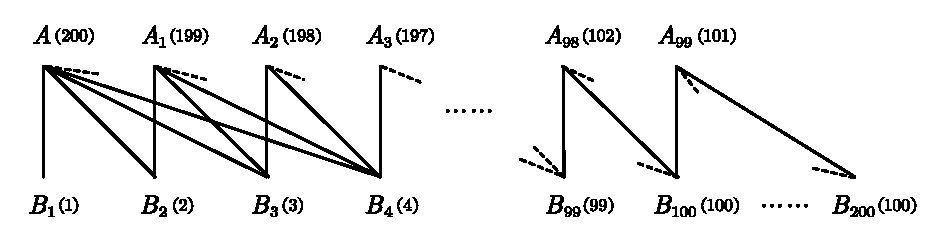
\includegraphics[width=14cm]{attachment/20230207.pdf}
	\end{center}
\end{solution}

\section{极端原理与无穷递降法}

\begin{instance}
	证明$\sqrt{2} \notin \mathbb{Q}$.
\end{instance}
\begin{solution}
	\begin{guess}
		设$\sqrt{2}=\dfrac{p}{q}$,则$q^2=2p^2$\ce{->T[令$q=2q_1$]}$2q_1^2=p^2$\ce{->T[令$p=2p_1$]}$2p_1^2=q_1^2 \cdots$然而不能像这样无穷递降下去.
	\end{guess}
	假设$(p,q)$是满足$q^2=2p^2$且使得$p+q$最小的一组数,若令$q=2q_1$,则$p^2=2q_1^2$,故$(q_1,p)$也满足要求,然而$q_1+p<p+q$,这与假设矛盾,故不存在满足要求的一组数.
\end{solution}

\begin{example} % 兴趣二阶组合2.1
	\nd{1}已知对于任意$n$个互不相同的实数两两求和有$\dfrac{n(n-1)}{2}$种不同的求法.求正整数$n$,满足存在$n~(n \geq 3)$个互不相同的整数,使得这些数两两求和恰可构成$\dfrac{n(n-1)}{2}$个连续的正整数.
\end{example}
\begin{solution}
	\buzhou{1}证明有上界:不妨设这$n$个数满足$a_1< \cdots <a_n$,于是$a_1+a_2<a_1+a_3< \textit{something} <a_{n-2}+a_n<a_{n-1}+a_n$.这意味着$a_3-a_2=1,~a_{n-1}-a_{n-2}=1$.若$n-2>3$,则必有$a_2+a_{n-1} = a_3+a_{n-2}$,因此$n \leq 5$. \\
	\buzhou{2}证明上界内部分可取:当$n=5$时,有$a_3-a_2=1,~a_4-a_3=1$,因而$$a_1+a_2 < a_1+a_3 < a_1+a_4 < \textit{something} < a_1+a_5 < \textit{something} <a_2+a_5 < a_3+a_5 < a_4+a_5$$
	其中两个\textit{something}的位置可以选择其一放置$a_2+a_3 < a_2+a_4 < a_3+a_4$.于是可知$(a_4+a_5) - (a_1+a_4)=7$,即$a_5-a_1=7$. \\
	若放在第一个位置,可得$a_2+a_3=a_1+a_4+1,~a_1+a_5=a_3+a_4+1$,解得$a_5=a_1+8$,矛盾; \\
	若放在第二个位置,可得$a_2+a_3=a_1+a_5+1,~a_2+a_5=a_3+a_4+1$,解得$a_5=a_1+8$,矛盾. \\
	因此,$n=5$时不合题意. \\
	另一方面,容易验证,当$n=3,4$时分别取
	$$(a_1,a_2,a_3) = (a_1,a_1+1,a_1+2)$$
	$$(a_1,a_2,a_3,a_4) = (a_1,a_1+1,a_1+2,a_1+4)$$
	可符合题意.综上,$n=3~ \textit{或} ~4$.
\end{solution}

\part{数论部分}


\end{document}





















